\phantomsection

\chapter{Resultados}\label{ch:capitulo_resultados}

Este capítulo apresenta os sinais e valores obtidos no experimento realizado no dispositivo de flexão.
Os tópicos aqui analisados apresentam a comparação dos resultados obtidos pelo experimento realizado pelo autor com os valores obtidos pelo
estudo de caso feito por Minela (2017).

O objetivo primário da comparação dos resultados é o de se obter dados descritivos de performance do dispositivo desenvolvido em relação a um sistema de medição industrial
homologado, no final do capítulo são indicados as situações de melhor performance do protótipo.

\section{Sinais obtidos}

Os sinais captados pelo sistema de medição desenvolvido seguem um formato trapezoidal, onde as zonas iniciais e finais representam os momentos em que a viga não se encontrava
sob a aplicação da carga, e a zona intermediária representa a total aplicação da carga no dispositivo.

\subsection{Sinais de calibração}

A primeira etapa da utilização do dispositivo é definir os sinais de calibração, para isso é obtido as respostas de leitura do amplificador de sinal para a aplicação das cargas
de 0,138kg e 1,04kg, que representavam o menor e o maior peso disponível para o experimento, sem considerar as combinações.

O sinal obtido para a massa de 0,138kg é mostrada na \autoref{fig:410}, o valor médio obtido pela análise do sinal foi de 190 bits.

\begin{figure}[htb]
	\caption{\label{fig:410} Sinal obtido sem a aplicação de cargas no dispositivo}
	\begin{center}
		\includegraphics[width=\textwidth]{pictures/signals/cal_signal_1.png}
	\end{center}
	\fonte{O autor 2022}
\end{figure}

O sinal obtido para a carga de 1,04kg é mostrada na \autoref{fig:420}, o valor médio obtido pela análise do sinal foi de 612 bits.

\begin{figure}[htb]
	\caption{\label{fig:420} Sinal obtido pela aplicação da cargas de calibração alta}
	\begin{center}
		\includegraphics[width=\textwidth]{pictures/signals/cal_signal_2.png}
	\end{center}
	\fonte{O autor 2022}
\end{figure}

Uma vez obtidos os valores em bits para cada ponto de calibraçãi e conhecidos os seus valores de deformação teóricos, é calculado os fatores "a" e "b" da função de interpolação
linear que converte valores obtidos pelo amplificador de sinal em bits para valores equivalentes de deformação no extensômetro.
O valor do fator a encontrado foi de $2.8881 bits/{\mu}m$ e o de b foi de $-363{\mu}m$.

Uma vez definidos os parâmetros de calibração são feitos os experimentos aplicando a carga de cada peso no dispositivo de flexão.
Alguns dos sinais obtidos e uma discussão geral sobre eles são discutidos nas seções a seguir.

\subsection{Sinais obtidos}

O sinal da menor carga aplicada é mostrada na \autoref{fig:4102},

\begin{figure}[H]
	\caption{\label{fig:4102} Sinal obtido da aplicação de 0,138 kg de carga aplicada no dispositivo}
	\begin{center}
		\includegraphics[width=\textwidth]{pictures/signals/w1.png}
	\end{center}
	\fonte{O autor 2022}
\end{figure}


%\begin{figure}[H]
%	\caption{\label{fig:4103} Sinal obtido da aplicação de 0,250 kg de carga aplicada no dispositivo}
%	\begin{center}
%		\includegraphics[width=\textwidth]{pictures/signals/w2.png}
%	\end{center}
%	\fonte{O autor 2022}
%\end{figure}
%
%\begin{figure}[H]
%	\caption{\label{fig:4104} Sinal obtido da aplicação de 0,337 kg de carga aplicada no dispositivo}
%	\begin{center}
%		\includegraphics[width=\textwidth]{pictures/signals/w3.png}
%	\end{center}
%	\fonte{O autor 2022}
%\end{figure}
%
%\begin{figure}[H]
%	\caption{\label{fig:4105} Sinal obtido da aplicação de 0,549 kg de carga aplicada no dispositivo}
%	\begin{center}
%		\includegraphics[width=\textwidth]{pictures/signals/w4.png}
%	\end{center}
%	\fonte{O autor 2022}
%\end{figure}
%
%\begin{figure}[H]
%	\caption{\label{fig:4106} Sinal obtido da aplicação de 0,636 kg de carga aplicada no dispositivo}
%	\begin{center}
%		\includegraphics[width=\textwidth]{pictures/signals/w5.png}
%	\end{center}
%	\fonte{O autor 2022}
%\end{figure}
%
%\begin{figure}[H]
%	\caption{\label{fig:4107} Sinal obtido da aplicação de 0,748 kg de carga aplicada no dispositivo}
%	\begin{center}
%		\includegraphics[width=\textwidth]{pictures/signals/w6.png}
%	\end{center}
%	\fonte{O autor 2022}
%\end{figure}
%
%
%\begin{figure}[H]
%	\caption{\label{fig:4108} Sinal obtido da aplicação de 0,834 kg de carga aplicada no dispositivo}
%	\begin{center}
%		\includegraphics[width=\textwidth]{pictures/signals/w7.png}
%	\end{center}
%	\fonte{O autor 2022}
%\end{figure}
%
%


\begin{figure}[H]
	\caption{\label{fig:4109} Sinal obtido da aplicação de 1,040 kg de carga aplicada no dispositivo}
	\begin{center}
		\includegraphics[width=\textwidth]{pictures/signals/w8.png}
	\end{center}
	\fonte{O autor 2022}
\end{figure}


%
%
%\begin{figure}[H]
%	\caption{\label{fig:4110} Sinal obtido da aplicação de 1,135 kg de carga aplicada no dispositivo}
%	\begin{center}
%		\includegraphics[width=\textwidth]{pictures/signals/w9.png}
%	\end{center}
%	\fonte{O autor 2022}
%\end{figure}
%
%\begin{figure}[H]
%	\caption{\label{fig:410} Sinal obtido da aplicação de 1,250 kg de carga aplicada no dispositivo}
%	\begin{center}
%		\includegraphics[width=\textwidth]{pictures/signals/w10.png}
%	\end{center}
%	\fonte{O autor 2022}
%\end{figure}
%
%\begin{figure}[H]
%	\caption{\label{fig:4111} Sinal obtido da aplicação de 1,330 kg de carga aplicada no dispositivo}
%	\begin{center}
%		\includegraphics[width=\textwidth]{pictures/signals/w11.png}
%	\end{center}
%	\fonte{O autor 2022}
%\end{figure}



%A \autoref{fig:4010} mostra os valores nominais de deformação para cada leitura da zona intermediária de cada sinal para cada combinação de cargas
%realizadas na execução do experimento, assim como o valor médio das amostras para cada combinação e o desvio padrão dos dados na zona intermediária
%de cada sinal como avaliação dos ruídos presentes.
%
%\begin{figure}[htb]
%	\caption{\label{fig:4010} Amostras e valores médios obtidos}
%	\begin{center}
%		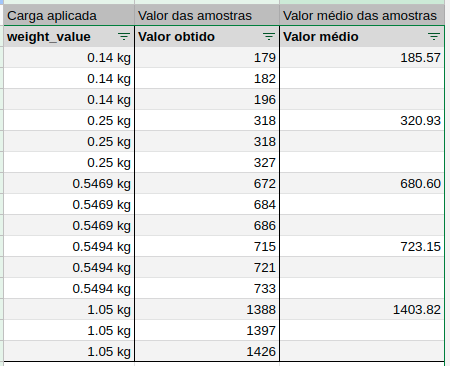
\includegraphics[width=\textwidth]{pictures/val_func_cal.png}
%	\end{center}
%	\fonte{O autor 2022}}
%\end{figure}

%Os Valores de carga compensados pelo problema da porca e do peso não encontrados conforme indicado na \autoref{}, junto com a comparação dos resultados obtidos por
%\autocite{Minela2017} são mostrados na \autoref{}.

%\section{Comparação final}
%
%A \autoref{} compara os principais resultados obtidos pelo experimento desenvolvido pelo autor com os resultados obtidos pelo trabalho de \autocite{Minela2017}.


%% TODO IMAGENS DE CARGAS


